\documentclass[12pt]{report}

\usepackage{commands}


\begin{document}

\large

\begin{center}
 Math 568 Homework 8\\
 Due 03/08/23\\
 By Marvyn Bailly\\
\end{center}

\normalsize

\hrule

%---------------%
%---Problem 1---%
%---------------%

%--status--$

\def\w{{\omega}}

\begin{problem}
    Consider the inverted pendulum dynamics:
    \begin{equation*}
        y'' + \paren{\delta + \eps \cos(\w t)}\sin(y) = 0.
    \end{equation*} 
    \begin{enumerate}
        \item[(a)] Perform a Floquet analysis of the pendulum with continuous forcing $\cos(\w t)$. 
        \item[(b)] Evaluate for what values of $\delta, \eps, \and \w$ the pendulum is stabilized.
    \end{enumerate}
\end{problem}

\begin{solution}
    \begin{enumerate}
        \item [(a)]
        \noindent
        Consider the pendulum dynamics given by,
        \begin{equation*}
            y'' + \paren{\delta + \eps \cos(\w t)}\sin(y) = 0.
        \end{equation*}
        When the pendulum is in the upright position, we can use Taylor expansion on the $\sin(x)$ to approximate the dynamics of the linear pendulum. In the inverted position (when $x = \pi$), we have the equation 
        \[ 
            y'' - \paren{\delta + \eps \cos(\w t)}y = 0,
        \]
        and in the downward (when $x = 0$) position by
        \[ 
            y'' + \paren{\delta + \eps \cos(\w t)}y = 0.
        \]
        To preform Floquet analysis, recall that the Floquet discriminant is of the form
        \[ 
            \Gamma = x_1\paren{\frac{2\pi}{\w}} + x_2'\paren{\frac{2\pi}{\w}}.
        \]
        where the solutions $x_1(t) \and x_2(t)$ satisfy the initial conditions
        \begin{align*}
            &y_1(0) = 1, \and y_1'(0) = 0,\\
            &y_2(0) = 0, \and y_2'(0) = 1.
        \end{align*} 
        If we let $v = y'$ and $u = y$, then we have the following system of equations
        \begin{align*}
            u' &= \mp \paren{\delta + \eps\cos(\w t)}v,\\
            v' &= u,
        \end{align*}
        which we can analyze in MATLAB. Using the code in Listings 1, we can generate the following plots:
        \begin{figure}[H]
            \begin{subfigure}[b]{0.5\linewidth}
                \centering
                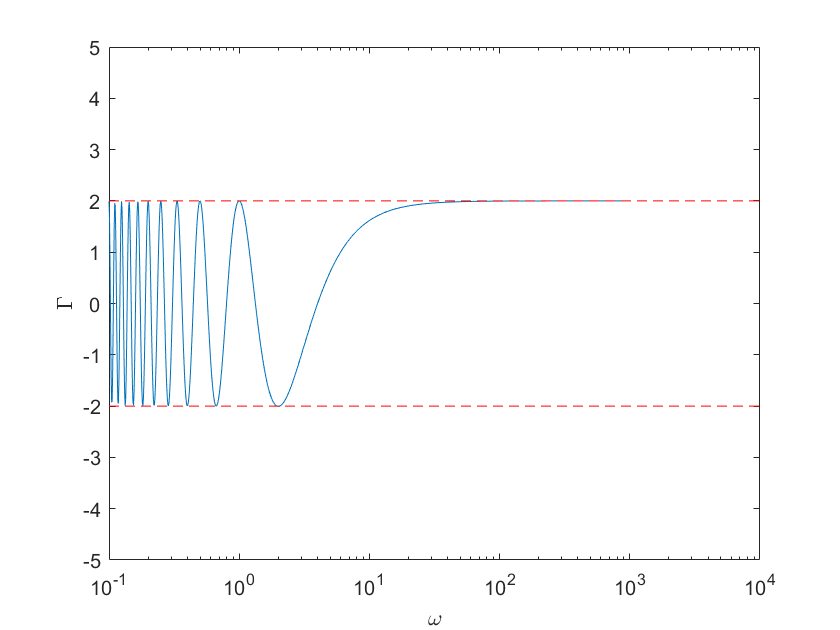
\includegraphics[width=\linewidth]{images/d1.png}
                \caption{Plot of downward pendulum using $\delta > \eps$.}
                \label{fig1:a}
                \vspace{4ex}
            \end{subfigure}%%
            \begin{subfigure}[b]{0.5\linewidth}
                \centering
                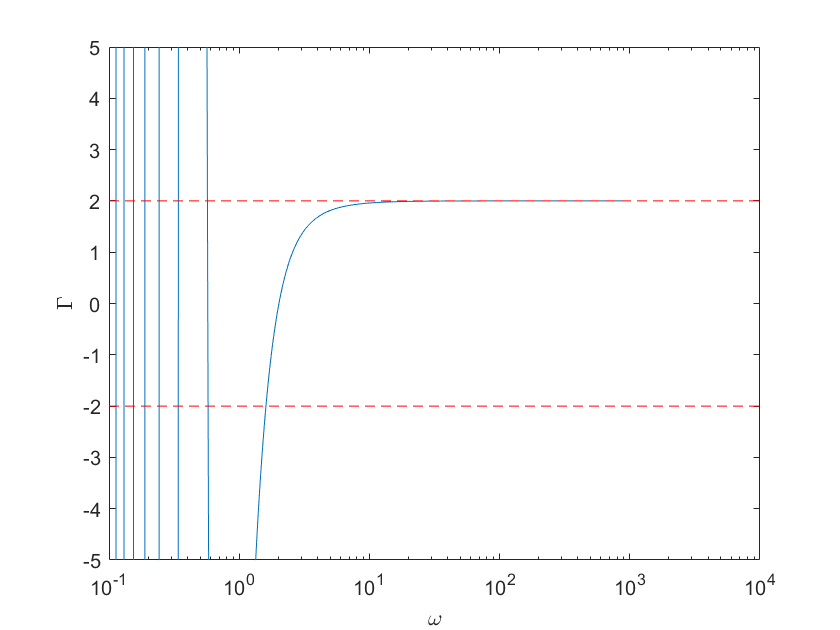
\includegraphics[width=\linewidth]{images/d2.png}
                \caption{Plot of downward pendulum using $\delta < \eps$}
                \label{fig1:b}
                \vspace{4ex}
            \end{subfigure}
            \caption{Plots of $\Gamma$ (blue solid line) for different $\w$ values in the downward pendulum. We also plot the stability boundaries where $\Gamma = \pm 2$ in the dotted red lines. In (a) we use $\delta = 1$ and $\eps = 0.1$ and (b) we use $\delta = 0.1$ and $\eps = 1$. }
            \label{fig1}
        \end{figure}
        \begin{figure}[H]
            \begin{subfigure}[b]{0.5\linewidth}
                \centering
                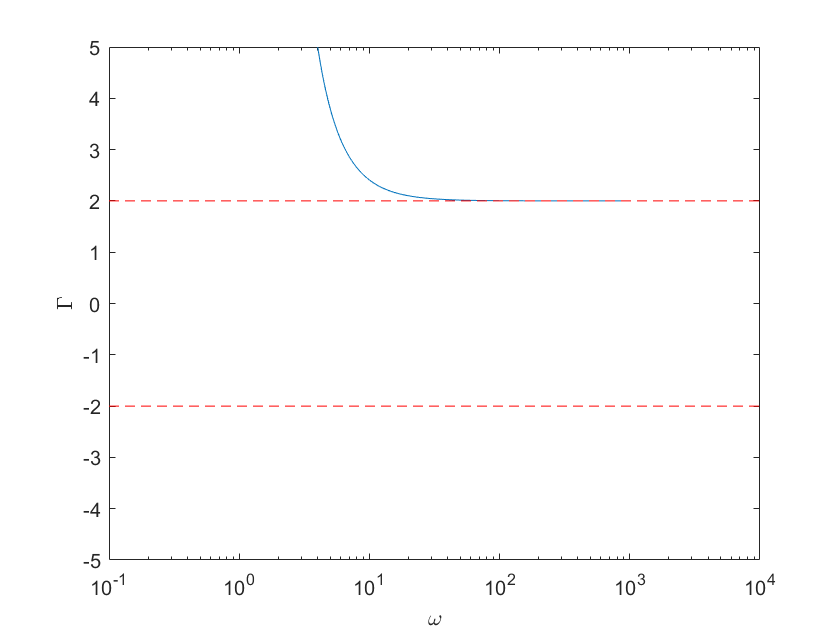
\includegraphics[width=\linewidth]{images/u1.png}
                \caption{Plot of upward pendulum using $\delta > \eps$.}
                \label{fig2:a}
                \vspace{4ex}
            \end{subfigure}%%
            \begin{subfigure}[b]{0.5\linewidth}
                \centering
                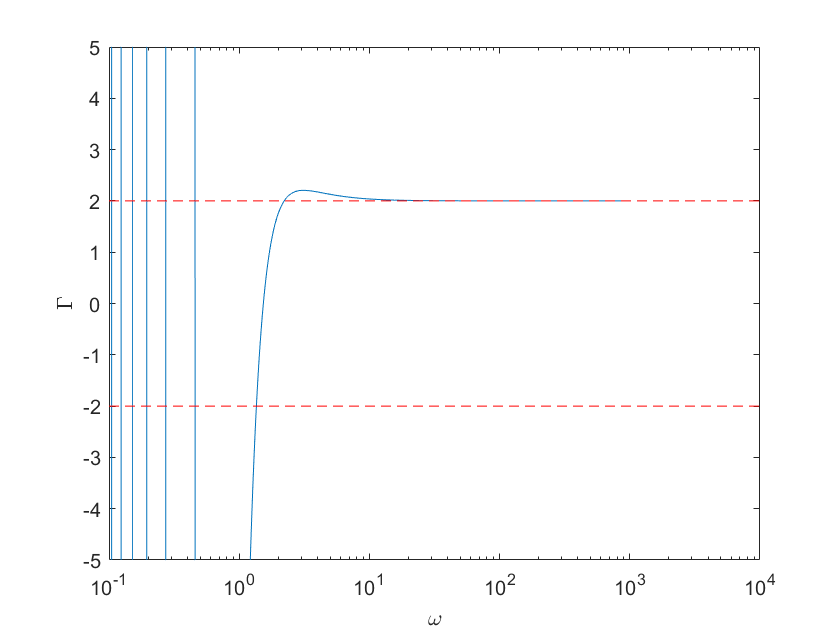
\includegraphics[width=\linewidth]{images/u2.png}
                \caption{Plot of upward pendulum using $\delta < \eps$}
                \label{fig2:b}
                \vspace{4ex}
            \end{subfigure}
            \caption{Plots of $\Gamma$ (blue solid line) for different $\w$ values in the upward pendulum. We also plot the stability boundaries where $\Gamma = \pm 2$ in the dotted red lines. In (a) we use $\delta = 1$ and $\eps = 0.1$ and (b) we use $\delta = 0.1$ and $\eps = 1$. }
            \label{fig2}
        \end{figure}
        \noindent
        For the nonlinear case, we follow a similar process but now using the equations
        \begin{align*}
            u' &= \mp \paren{\delta + \eps\cos(\w t)}\sin(v),\\
            v' &= u.
        \end{align*}    
        Using MATLAB, we can generate the following plots:
        \begin{figure}[H]
            \begin{subfigure}[b]{0.5\linewidth}
                \centering
                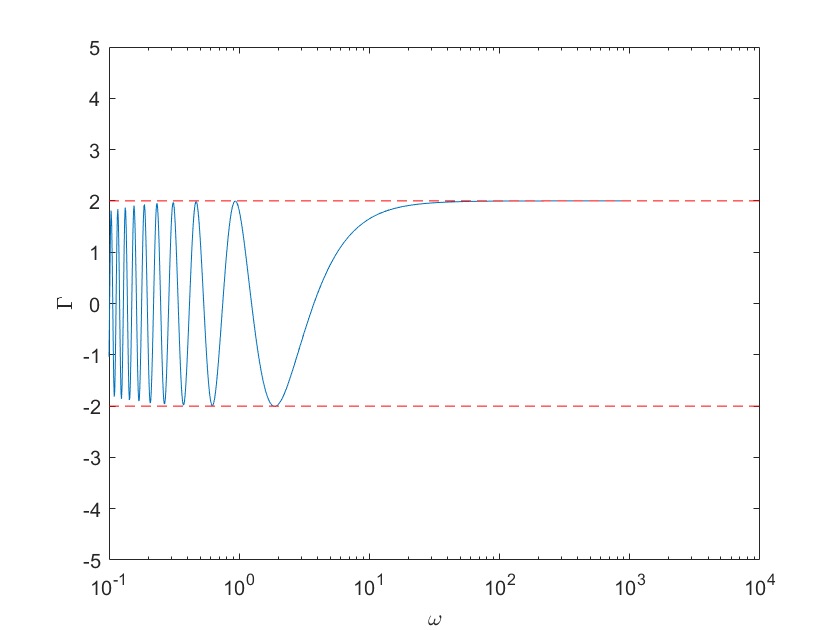
\includegraphics[width=\linewidth]{images/nld1.png}
                \caption{Plot of downward pendulum using $\delta > \eps$.}
                \label{fig3:a}
                \vspace{4ex}
            \end{subfigure}%%
            \begin{subfigure}[b]{0.5\linewidth}
                \centering
                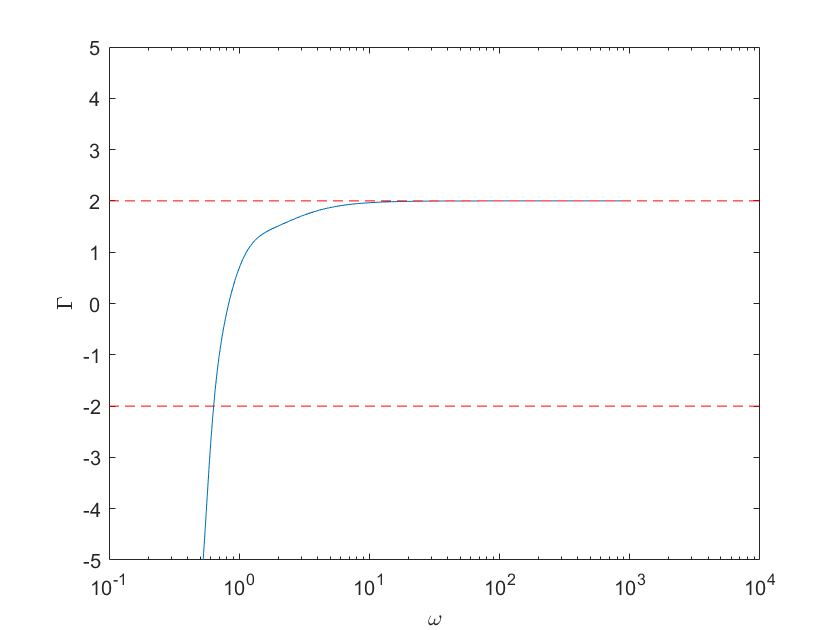
\includegraphics[width=\linewidth]{images/nld2.png}
                \caption{Plot of downward pendulum using $\delta < \eps$}
                \label{fig3:b}
                \vspace{4ex}
            \end{subfigure}
            \caption{Plots of $\Gamma$ (blue solid line) for different $\w$ values in the downward pendulum. We also plot the stability boundaries where $\Gamma = \pm 2$ in the dotted red lines. In (a) we use $\delta = 1$ and $\eps = 0.1$ and (b) we use $\delta = 0.1$ and $\eps = 0.2$. }
            \label{fig3}
        \end{figure}
        \begin{figure}[H]
            \begin{subfigure}[b]{0.5\linewidth}
                \centering
                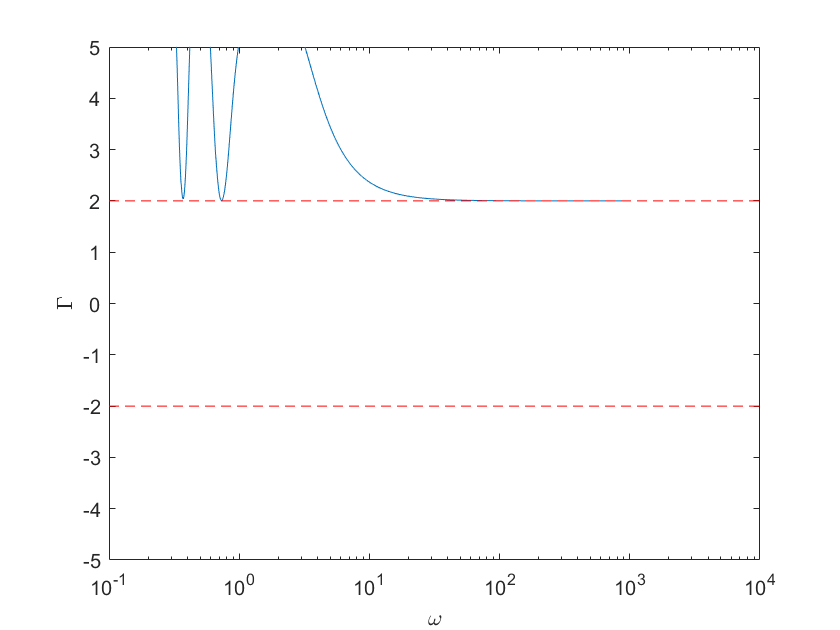
\includegraphics[width=\linewidth]{images/nlu1.png}
                \caption{Plot of upward pendulum using $\delta > \eps$.}
                \label{fig4:a}
                \vspace{4ex}
            \end{subfigure}%%
            \begin{subfigure}[b]{0.5\linewidth}
                \centering
                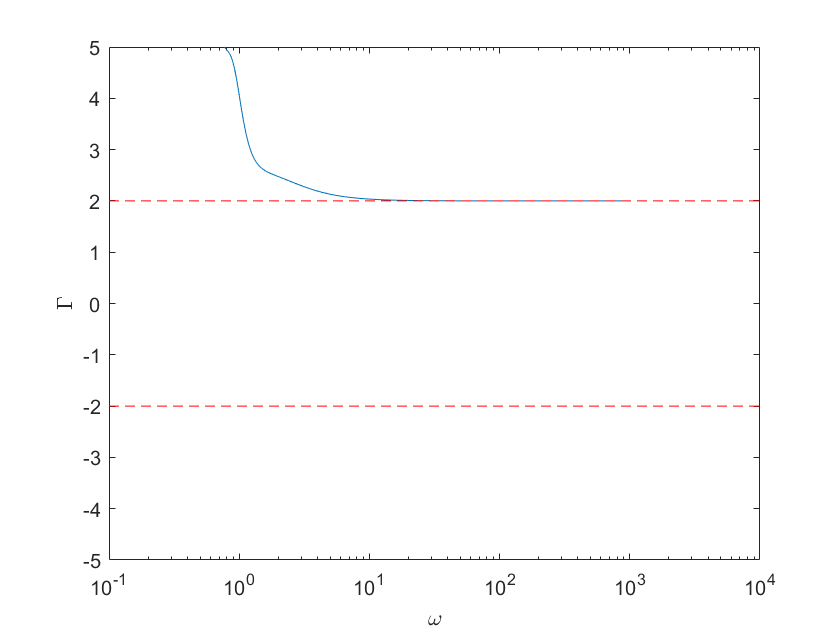
\includegraphics[width=\linewidth]{images/nlu2.png}
                \caption{Plot of upward pendulum using $\delta < \eps$}
                \label{fig4:b}
                \vspace{4ex}
            \end{subfigure}
            \caption{Plots of $\Gamma$ (blue solid line) for different $\w$ values in the upward pendulum. We also plot the stability boundaries where $\Gamma = \pm 2$ in the dotted red lines. In (a) we use $\delta = 1$ and $\eps = 0.1$ and (b) we use $\delta = 0.1$ and $\eps = 1$. }
            \label{fig4}
        \end{figure}







        
        \item [(b)]
        To find where the pendulum is stable, we can look at the Figures 1,2,3, and 4 and see when $\Gamma$ is less than $|2|$. 



    \end{enumerate}
    



    \lstinputlisting[language=MATLAB, caption={\bf MATLAB code used to generated plots.}]{hw8.m}
\end{solution}

%----------------------------------------------------------------------------------------------------%
%\vskip 20pt
\newpage


\end{document}